% This is the project description we were provided we can tailor it later
Silicate glasses are very important materials in fields including medicine, optics, electronics, telecommunication and energy. The unique mechanical and thermal properties of these glasses are well documented but one of the main limitations are anomalies in the silicate structure that cause fractures to occur. Figure \ref{crack_prop} shows a 2D visualization of this mechanism. Given that glass is extremely brittle, fractures may occur instantaneously when a maximum stress level is reached \cite{pedone2015dynamics}. Predicting and modeling these fractures mechanisms has been a researched extensively.





\begin{comment}
\begin{figure}[!h]
  \centering
  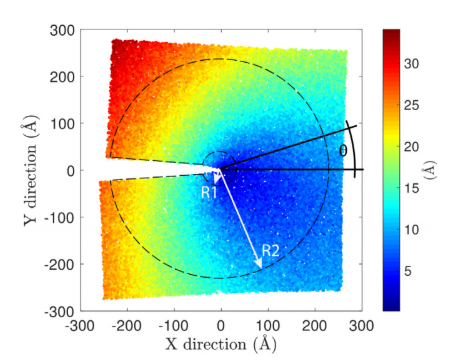
\includegraphics[width=11cm]{picture/FractureMechanism2.PNG}
  \caption{Configuration showing the coordinate axes and crack tip relationship similar to the Williams expansion. Dashed lines show an annulus
with inner radius R1 and outer R2. Points are colored according to the magnitude of their displacement under an applied field. Figure reproduced from~\protect\cite{mWilson_continuum_stress}} 
  \label{crack_rad2}
\end{figure}

\end{comment}

Nucleation of fractures originates from defects of the atomic structure of silicate glass. 
The fractures do not necessarily occur when the weakest bond in the structure breaks and triggers numerous other breaks in the surrounding bonds. Instead, the fracturing is dependent on the local structure surrounding the atoms so defining this relation is critical in the fracture analysis. While these relations can be studied using results from MD, a repetitive simulation-observation approach is computationally prohibitive. A more tractable approach is to use machine learning and surrogate modeling techniques.

\begin{figure}
    \centering
    \noindent
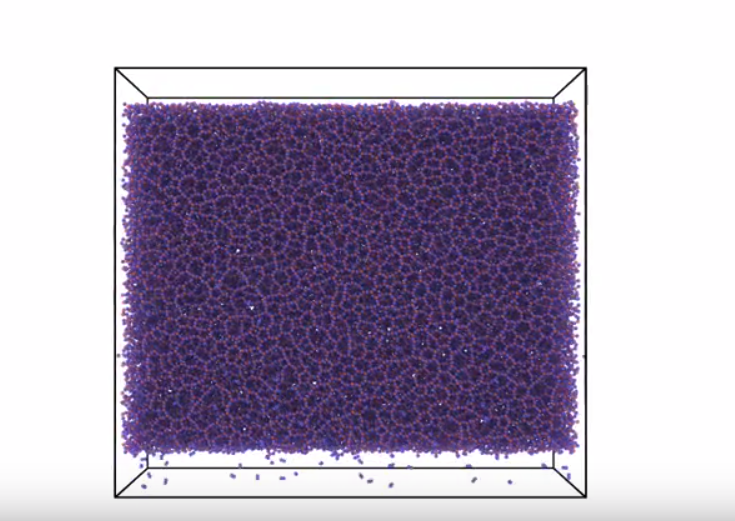
\includegraphics[width=0.4\textwidth]{picture/frac_prop1.PNG}\hspace{0.2\textwidth}%
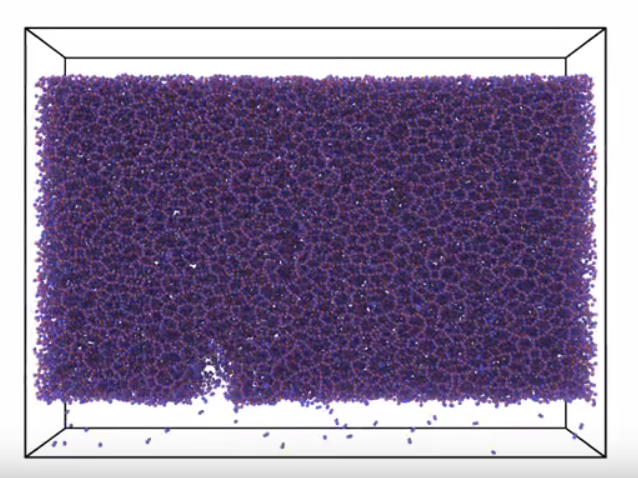
\includegraphics[width=0.4\textwidth]{picture/frac_prop2.PNG}\\[2em]
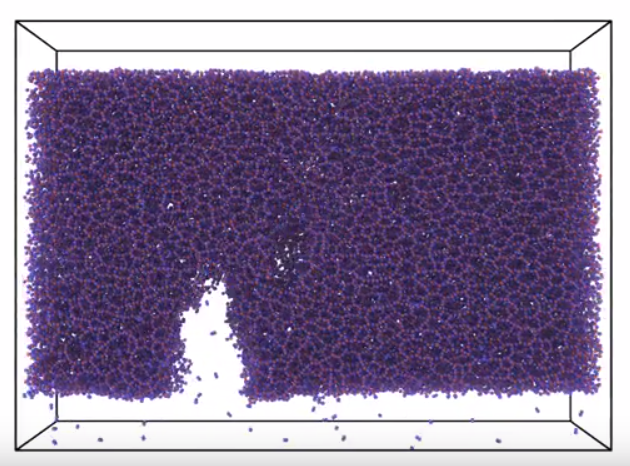
\includegraphics[width=0.4\textwidth]{picture/frac_prop3.PNG}\hspace{0.2\textwidth}%
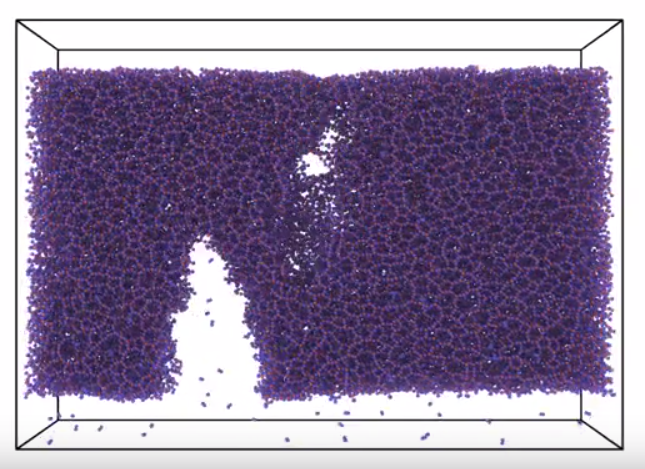
\includegraphics[width=0.4\textwidth]{picture/frac_prop4.PNG}\par

    \caption{Crack propagation}
    \label{crack_prop}
\end{figure}


\begin{comment}
\begin{figure}[!b]
  \centering
  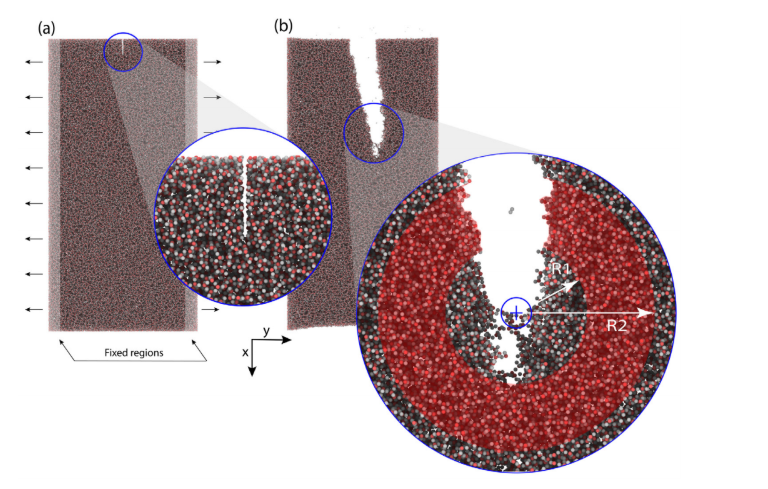
\includegraphics[width=11cm]{picture/FractureMechanism.PNG}
  \caption{Images of a simulated a-SiO2 sample. (a) Samples are loaded and held in mode I tension. Initial cracks are created by removing a
small number of atoms from the upper surface of the sample. (b) An example of crack propagation in a loaded sample, with the crack tip
identified by the +, and the annulus colored red. Figure reproduced from~\protect\cite{mWilson_continuum_stress}} 
  \label{crack_prop2}
\end{figure}
\end{comment}





Typically in these silicate glass structures, silicon (Si) is surrounded by four oxygen (O) atoms forming a tetrahedron seen in Figure \ref{SiO2}. These tetrahedra share one common O atom if they are neighbors. A ring forms if a group of tetrahedra share common O atoms, and the size of these rings is computed based on how many Si atoms are in the ring. A large ring has 11 and 12 Si atoms, medium rings have 5 and 6, and small rings have 1 or 2.

\begin{figure}[!h]
  \centering
  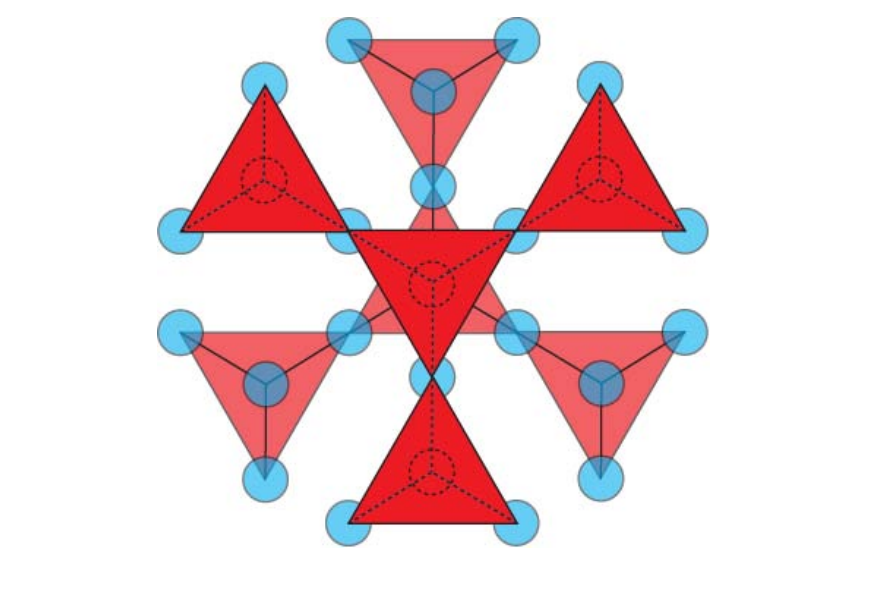
\includegraphics[width=11cm]{picture/SiO2Ring.PNG}
  \caption{SiO2 Ring structure
Figure reproduced from UMass Amherst Dept. Geosciences} 
  \label{SiO2}
\end{figure}

\begin{comment}
It was also shown that increasing the quenching rates, increased the number of large-sized rings and decreased the number of medium-sized rings decreases \cite{ebrahem2018influence}. The change in the number of small-sized rings was minimal. And because there is larger void in large-sized ring, it can be stretched and deformed more than the medium-sized ring. However, medium-sized ring can take more per unit stress while tensile is applied, so it has more strain energy.

\end{comment}



%%%%%%%%%%%

\begin{comment}
An atom is denoted as under-coordinated if the number of its constraints is lower than 4, and over-constrained, if greater than 4\cite{pedone2015dynamics}. 

\end{comment}
%%%%%%%%%%%%%%%%%

Classical molecular dynamics simulations were also used to investigate the properties of silicate glasses. Glasses were observed using 60k atoms for soda-silicate glasses and 30k atoms for silica glass \cite{pedone2015dynamics}. Soda-lime silicate glasses were analyzed at the nanometric scale with an atomic force microscope. Cavities were formed at 20nm long and 5nm deep ahead of the crack tip, and cracks would advance following the coalescence of cavities \cite{pedone2015dynamics}.

Regarding the mechanical properties of the silicate glass, Young's modulus, strength, failure strain and fracture mechanism were all used throughout the study \cite{pedone2015dynamics}.  Additionally, these properties depend on both the strain rate and the quench rate. The glasses were heated at 5000 K, a temperature considered more than adequate to bring the glass into a liquid state and the heat was equilibrated for 100 picoseconds and then cooled continuously to 300 K with a normal cooling rate of 5 K/ps. \cite{pedone2015dynamics}.

With regards to stress, uniaxial tensile tests were implemented along the z-axis for both bulk glasses and nanowires \cite{pedone2015dynamics}. An important finding is such that for uniaxial tension tests in bulk glasses, in particular flaw-free silica glass, the glass was forced to break in a brittle manner \cite{pedone2015dynamics}. Additionally, in flaw-free glass, voids would grow, then coalesce before the structure would fracture. What was concluded as a result of the numerous tests performed was that the fracture mechanism of defective models showed to be less brittle compared to flaw-free glass given the unstable region is capable of expansion \cite{pedone2015dynamics}. This is an important finding given that it contradicts what is generally expected of silicate glasses.\cite{radialDistribution}


